
%---------------------------------------------------------------------------------------------------------
%-
%-                                                Calibration class description
%-
%----------------------------------------------------------------------------------------------------------
\section{Description of the calibration classes}
In this chapter the working principles of the three calibration classes ``AliTPCCalibPedestal'', ``AliTPCCalibPulser'' and ``AliTPCCalibCE'' will be explained in detail. After an introduction about the commonalities of the classes (interface, work flow), each algorithm will be on its own.

\subsection{Common introduction}
The general idea of the calibration classes is to process and analyse raw data. The algorithms are supposed to run in different environments, such as in the offline reconstrution, the high level trigger or in the data acquisition system.
% \subsection{Event processing}
To guarantee flexibility in the data processing, several methods are available calling each other in a hirachical order. For the decoding of the raw data two different algorithms are available which led to two branches of processing functions.
The relavent functions are called {\bf ProcessEvent[Fast]} taking as an input either the DATE  {\bf eventHeaderStruct} an {\bf AliRawReader} object or an {\bf AliTPCRawStream[Fast]} object.
The function which does the actual processing of the data is called {\bf Upate} and takes as arguments the sector, pad row, pad, time bin and adc signal. All this is summariesed in fig.\ \ref{fig:calib.process}.

\begin{figure}
  \centering
  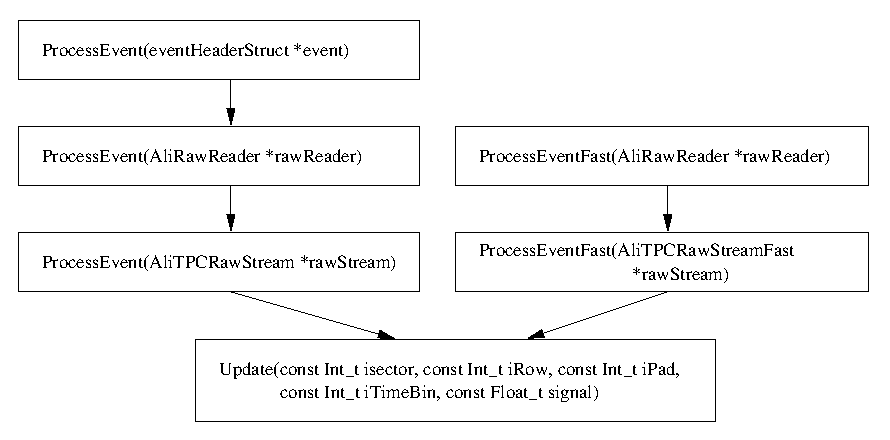
\includegraphics[width=0.9\linewidth]{images/ProcessFunctions}
  \caption{Hirachy of the event processing functions of the calibration algorithms.}
  \label{fig:calib.process}
\end{figure}

The calibration data is stored in {\em reference histograms}, filled in the {\bf Update} function, functions called inside, and the {\bf EndEvent} function. For each readout chamber and calibration variable {\it XXX} one reference histogram is created. These are two dimensional having on the y-axis the channel number within the ROC and on the x-axis the distribution of the calibration variable. Setters exist to adjust the range and number of bins. An example of a reference histogram can be found in fig.\ \ref{app:calib.refhist}.

Inside the calibration class the reference histograms are stored in {\em TObjArrays}, one for each variable keeping the 72 histograms for the ROCs. The arrays are called {\bf fHisto{\it XXX}Array} and can be retrieved with the getter function {\bf GetHisto{\it XXX}}(Int\_t sector, Bool\_t force=kFALSE). To allocate memory only if needed, the histograms are created the first time the getter is called and the force flag is set to kTRUE.

\begin{figure}
  \centering
  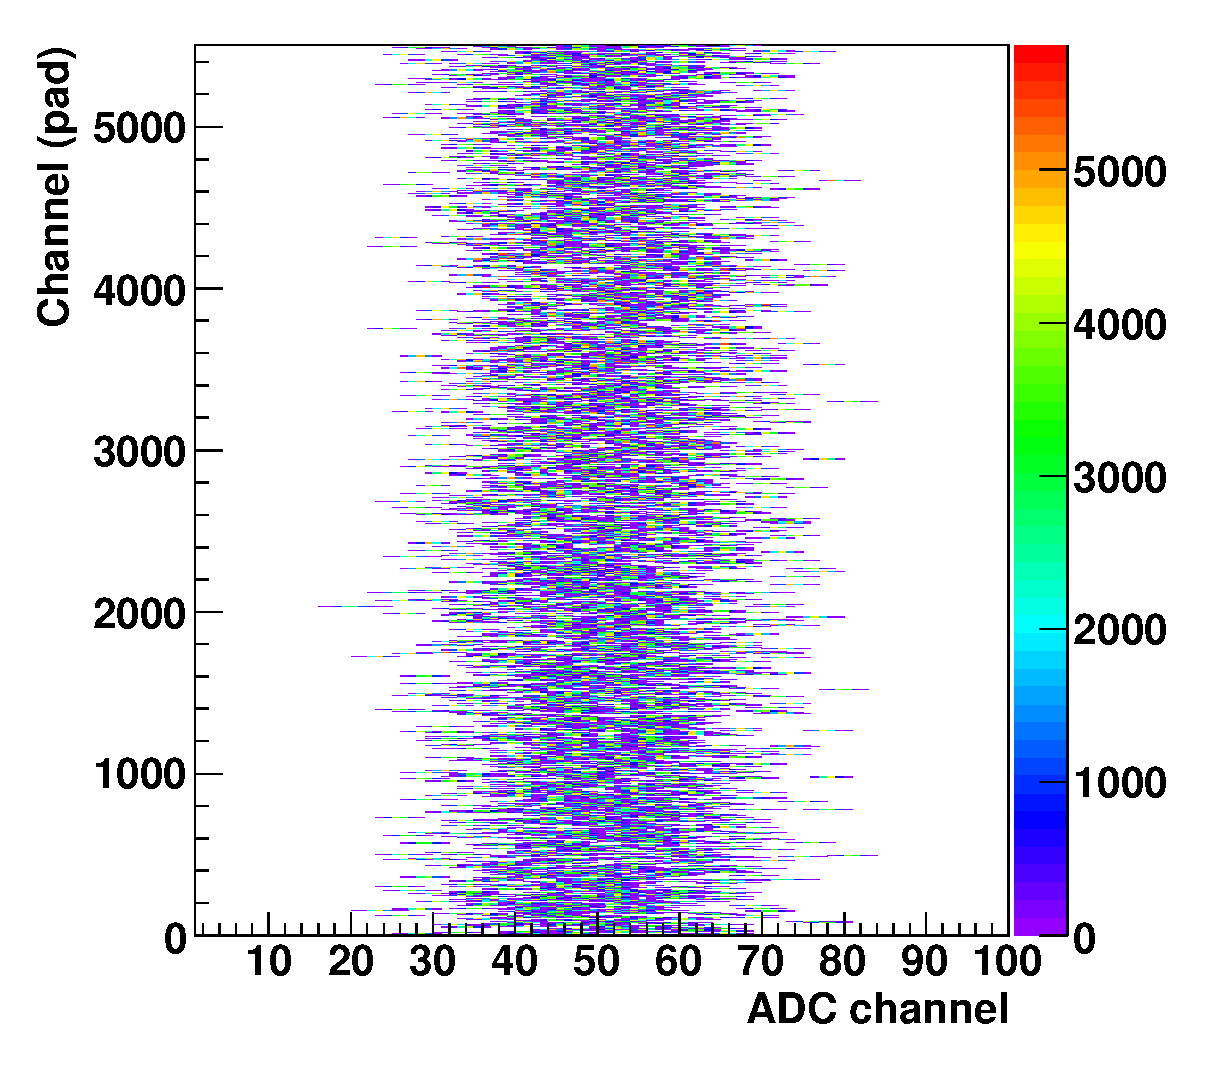
\includegraphics[width=7.3cm]{images/RefHist}
  \caption{Example of a reference histogram. Displayed are the electronic baseline distributions for all pads of one IROC.}
  \label{fig:calib.refhist}
\end{figure}

For the Pulser and CE calibration after each event the {\bf EndEvent function} has to called, doing some post processing, the filling of a part of the reference histograms and calculation of data stored event by event (see description below).

After the desired statistics has been accumulated the actual calibration values pad by pad are calculated by calling the {\bf Analyse} function. To store the data a special class {\bf AliTPCCalROC} is used keeping all values for one readout chamber. As in case of the reference histograms, the AliTPCCalROC objects are only created upon request, by using the getter function {\bf GetCalRoc{\it XXX}}(Int\_t sector, Bool\_t force=kFALSE) with the force flag set to kTRUE. The objects are also stored in {\em TObjArrays} which are called {\bf fCalRocArray{\it XXX}}. A pointer the complete arrays is provided by the {\bf GetCalPad{\it XXX}}() functions.

To save the calibration data the function {\bf DumpToFile} is available, taking as arguments the filename and optional a directory name to which it should be stored in the file and if the file should be updated instead of overwritten.

The process flow described above is summarised in fig.\ \ref{fig:calib.calibflow}

\begin{figure}
  \centering
  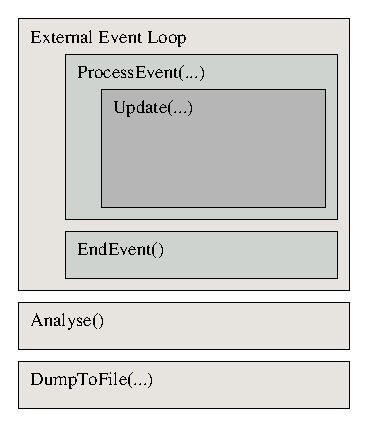
\includegraphics[width=7cm]{images/ProcessFlow}
  \caption{Process flow of the calibration algorithms.}
  \label{fig:calib.calibflow}
\end{figure}

%################################################################################
\subsection{Pedestal calibration class}
\subsubsection{Signal filling {\small [Update(\dots)]}}
The {\bf Update} function fills the reference histograms with the ADC values of all time bins in the selected range (fFirstTimeBin, fLastTimeBin) with standard values (60, 1000). The range can be specified by the setter function {\bf SetRangeTime}(Int\_t tMin, Int\_t tMax).
If requested by {\bf SetTimeAnalysis}(Bool\_t time = kTRUE), pedestal values for each time bin will be calculated. This information can be used to fill the pattern memory of the ALTRO in order to perform a timebin by timebin baseline subsection.

\subsubsection{Calibration value calculation {\small [Analyse()]}}
Calling the {\bf Analyse}() routine calculates the pedestal and noise values for each channel by fitting a gaus function on the distribution. In addition a second approach is used calculating the mean and corresponding RMS. If desired a truncation range can be set using the {\bf SetAnalysisTruncationRange}(Float\_t down, Float\_t up) function, where down and up mark the range as a fraction of the data: e.g. (0.05,0.9) would exclude the lower 5\% and upper 10\%.

\subsubsection{Stored calibration values}
The available calibration values calculated in the pedestal calibration class, a description as well as the corresponding getter functions are summariesed in table\ \ref{app:tab.pedestal}

\begin{table}[H]
  \footnotesize
  \centering
  \begin{tabular}{l|p{3.2cm}|l|l}
  \hline
  {\bf Cal. value} & {\bf description} & {\bf getter} {\scriptsize (AliTPCCalROC*)} & {\bf getter} {\scriptsize (TObjArray*)}\\
  \hline
  \hline
  Pedestal & pedestal value\newline {\footnotesize (mean of a gaus fit)}       & GetCalRocPedestal(sector) & GetCalPadPedestal() \\
  Sigma    & noise value\newline {\footnotesize (sigma of a gaus fit)}         & GetCalRocSigma(sector)    & GetCalPadSigma() \\
  Mean     & pedestal value\newline {\footnotesize (mean of the distribution)} & GetCalRocMean(sector)     & GetCalPadMean() \\
  RMS      & noise value\newline {\footnotesize (rms of the distribution)}     & GetCalRocRMS(sector)      & GetCalPadRMS() \\
  \hline
  \end{tabular}
  \caption{Calibration values}
  \label{app:tab.pedestal}
\end{table}

%################################################################################
\subsection{Pulser calibration class} \label{app:calib.pulser}
\subsubsection{Signal filling {\small [Update(\dots)]}} \label{app:calib.pulser.updated}
In the {\bf Upate}(\dots) function of the Pulser Calibration class an array (fPadSignal) is filled with the ADC signal information for each timebin of the currently processed channel (pad). In addition the maximum ADC value and corresponding timebin is stored (fMaxPadSignal, fMaxTimeBin). Only the selected time range (fFirstTimeBin, fLastTimeBin) is taken into account. The range can be set by calling {\bf SetRangeTime}(Int\_t firstTimeBin, Int\_t lastTimeBin). Before proceeding with the next channel, the {\bf ProcessPad}() function is called, which analyses the information currently stored in fPadSignal.

\subsubsection{Channel information processing {\small [ProcessPad()]}}
As a first step the pedestal and noise values for the current pad are queried ({\bf FindPedestal}()). Therefore either previouly measured data can be used ({\bf SetPedestalDatabase}(AliTPCCalPad *pedestalTPC, AliTPCCalPad *padNoiseTPC)) or if not set the pedestal and noise will be calculated. This is done by calculating the truncated mean and RMS within a range of $\pm 10$\,ADC channels around the median of the signal distribution stored in fPadSignal.

In the second step the properties of the pulser signal are calculated ({\bf FindPulserSignal}(\dots)). For the analysis it is assumed that there is only one signal which spreads over a range of minus two to plus seven timebins around fMaxTimeBin. After the pedestal substraction the signal sum, mean and RMS are calculated in this range. If the signal sum is below a threshold of 8 times the pad noise (minimum noise set to 1 ADC count), all values are set to zero.

As a third step the reference histograms for the charge (signal sum) and signal width information are filled. The time position (signal mean) is stored in an array for later processing (see below).

\subsubsection{Event information processing {\small [EndEvent()]}}
The {\bf EndEvent}() function loops over all readout chambers and filles the time information into the reference histograms. Stored is the deviation from the mean of the time signals in the currently processed ROC.

\subsubsection{Calibration value calculation {\small [Analyse()]}}
In the {\bf Analyse}() function the final calibration values are calculated as the mean of the distributions stored in the reference histograms. The information is finally stored in AliTPCCalROC objects.

\subsubsection{Stored calibration values}
The available calibration values calculated in the pulser calibration class, a description as well as the corresponding getter functions are summariesed in table\ \ref{app:tab.pulser}

\begin{table}[H]
  \footnotesize
  \centering
  \begin{tabular}{l|p{3.2cm}|l|l}
  \hline
{\bf Calib. value} & {\bf description} & {\bf getter} {\scriptsize (AliTPCCalROC*)} & {\bf getter} {\scriptsize (TObjArray*)}\\
  \hline
  \hline
  T0  & time position {\footnotesize (relative to chamber mean)} & GetCalRocT0(sector) & GetCalPadT0() \\
  \hline
  Q   & signal sum          & GetCalRocQ(sector)    & GetCalPadQ() \\
  \hline
  RMS & signal width        & GetCalRocRMS(sector)  & GetCalPadRMS() \\
  \hline
  \end{tabular}
  \caption{Calibration values in the pulser calibration class}
  \label{app:tab.pulser}
\end{table}


\subsection{Central electrode signal calibration class}
\subsubsection{Signal filling {\small [Update(\dots)]}}
Before calling either the {\bf ProcessEvent}(\dots) or the {\bf Update}(\dots) function, {\bf SetEventInfo}(Double\_t runNumber, Double\_t timestamp, Double\_t eventId) should be called for each event to be able to display some of the stored calibration values as one a function of on of these information. The {\bf Update}(\dots) function itself is exactly the same as described above in the Calibration Pulser section (\ref{app:calib.pulser.updated}).

\subsubsection{Channel information processing {\small [ProcessPad()]}}
The first step is getting the pedestal and noise values (see \ref{app:calib.pulser.updated}).

In the second step local maxima are searched in the pad signal ({\bf FindLocalMaxima}(\dots).  For each chamber a histogram is filled with this information. To be accepted as a local maximum the signal has to be five times larger than the pad noise and needs 2(3) preceding (succeeding) timebins with a falling signal height. Maxima are expected to arise from the laser rays, photoelectrons from the central electrode, but also periodic post peaks following the CE signal have been observed. The largest fraction however arising from the CE. In the {\bf EndEvent}() function for each ROC the time position of the maximum of the local maxima distribution will be calculated, identified with the time position of the central electrode and stored event by event in an array ({\it fTMeanArrayEvent}).

If no event has been processed yet in this run no further processing on the pad signal will be done. The reason is that no position information of the central electrode signal is available at that point.

The third step is the analysis of the central electrode signal ({\bf FindCESignal}(\dots)). To decide which of the local maxima found before represents the CE signal, the distance to the identified position of the previous event (see end of second step) is calculated. The maximum with the smallest distance is used. Signal sum, mean and RMS are calculated in a range of -4 to +7 timebins around the maximum. If the signal sum is smaller than eight times the pad noise, all values will be set to zero.

The fourth step filling of the signal sum and width histograms, as well as filling a temporary array with the time (signal mean) information.

\subsubsection{Event information processing {\small [EndEvent()]}}
In the beginning of the function the mean drift time for each readout side is calculated.

Next it is looped over all sectors for which information are available. If the local maxima distribution histogram has less entries than 2/3 of the number of channels of the ROC, it will be skipped. This is the reason if the calibration algorithm is run on data which has no laser events.

As already described above the maximum position of the local maxima distribution is calculated. For this purpose the truncated mean within a range of $\pm4$ timebins around the median of the distribution is used.

To monitor the stability of the laser, the mean charge (signal sum) is calculated for each ROC and stored event by event.

In a loop over all channels the time reference histograms are filled with the difference of the pad time  signal to the mean arrival time of the corresponding readout side, calculated above. This approach is used to accumulate statistics over a long time range in which the drift velocity might change. Non time dependend and time dependend effects are such hoped to be decoupled to a large extent. In addition a temporary AliTPCCalROC object is filled with the time inforation.

The AliTPCCalROC object is used to perform a linear as well as parabolic 2D fit to the data. This information is stored event by event and can be used to study non uniform changes in the drift velocity.

\subsubsection{Calibration value calculation {\small [Analyse()]}}
In the {\bf Analyse}() function the final calibration values are calculated as the mean of the distributions stored in the reference histograms. The information is finally stored in AliTPCCalROC objects.

\subsubsection{Stored calibration values}
The available calibration values calculated in the pulser calibration class, a description as well as the corresponding getter functions are summariesed in table\ \ref{app:tab.ce}

\begin{table}[H]
  \centering
  \footnotesize
  \begin{tabular}{l|p{3.2cm}|l|l}
  \hline
{\bf Calib. value} & {\bf description} & {\bf getter} {\scriptsize (AliTPCCalROC*)} & {\bf getter} {\scriptsize (TObjArray*)}\\
  \hline
  \hline
  T0  & time position {\footnotesize (relative to the readout side)} & GetCalRocT0(sector) & GetCalPadT0() \\
  \hline
  Q   & signal sum          & GetCalRocQ(sector)    & GetCalPadQ() \\
  \hline
  RMS & signal width        & GetCalRocRMS(sector)  & GetCalPadRMS() \\
  \hline
  \end{tabular}
  \caption{Calibration values in the central electrode calibration class}
  \label{app:tab.ce}
\end{table}

As described above additional data is stored event by event for each chamber. Table \ref{app:tab.ceebye} summarieses the information, gives a short description and shows the getter function.
\begin{table}[H]
  \centering
  \footnotesize
  \begin{tabular}{p{4cm}|l|p{4cm}}
  \hline
{\bf type of information} & {\bf getter } & {\bf description} \\
\hline\hline
results of a plane fit  & GetParamArrayPol1(sector) & {\small returns a TObjArray of TVectorD objects, one entry per event}\\
\hline
results of 2D parabolic fit  & GetParamArrayPol2(sector) & {\small returns a TObjArray of TVectorD objects, one entry per event}\\
\hline
mean arrival time & GetTMeanEvents(sector) & returns an array of floats (TVectorF), one entry per event\\
\hline
mean signal sum & GetQMeanEvents(sector) & returns an array of floats (TVectorF), one entry per event\\
\hline
  \end{tabular}
  \caption{Event by event information stored for each chamber in the central electrode calibration class}
  \label{app:tab.ceebye}
\end{table}


\subsection{Using the Calibration Classes} \label{app:code.calib}
% \subsection{Data processing}
Listing \ref{app:code.fillcalib} shows an example how to loop over one root raw data file to fill one of the calibration classes for either Pedestal and Noise calibration, analysing data taken with the Calibration Pulser or retrieving information from the Central Electrode signal acquired from events using the TPC laser system.

The code shows a ROOT macro that is supposed to be executed from the commandline prompt in the ALICE offline analysis framework AliRoot. In the example {\em XXX} has to be replaced bei one of {\em Pedestal}, {\em Pulser} or {\em CE}.

Examples of how to load the macro and execute it is shown in listing \ref{app:code.pedestal} for the case of a pedestal run and \ref{app:code.pulserCE} in case of a pulser or laser run. The listings also demonstrate the possibility of displaying the stored calibration data using the AliTPCCalPad class. For more information see the documentation in the class code.

\CodeMacro{fillCalibObject.C}{app:code.fillcalib}
\CodeCint{commandsPedestal.cint}{app:code.pedestal}
\CodeCint{commandsPulserCE.cint}{app:code.pulserCE}
